\documentclass[polish, 11pt, a4paper]{article}

\usepackage{polski}
\usepackage[utf8]{inputenc}
\usepackage[autostyle]{csquotes}
\DeclareQuoteAlias{dutch}{polish}
\usepackage[T1]{fontenc}
\usepackage{geometry}
\geometry{
	a4paper,
	total={170mm,257mm},
	left=25mm,
	right=25mm,
	top=20mm,
}

\usepackage{babel}
\usepackage{microtype}
\usepackage{lmodern}
\usepackage{multirow}
\usepackage{makecell}
\usepackage{array}
\newcolumntype{?}[1]{!{\vrule width #1}}
\usepackage{amsmath}
\usepackage{caption}
\usepackage{graphicx}
\usepackage{graphics}
\usepackage{float}
\usepackage{enumitem}
\usepackage{ragged2e}
\usepackage{parskip}
\RaggedRightParindent = 24 pt
\usepackage{indentfirst}
\usepackage[figurename=Wykres]{caption}

\begin{document}
	\begin{titlepage}
	\centering
	\Huge Laboratorium Podstaw Fizyki\\
	\vspace{1cm}
	\huge Ćwiczenie 104 \enquote{Efekt fotowoltaiczny - ogniwo słoneczne}\\
	\vspace{1cm}
	\raggedright
	\huge Prowadzący: mgr Karolina Paradowska\\
	\vspace{.5cm}
	\begin{table}[h]
		\centering
		\resizebox{\columnwidth}{!}{%
		\begin{tabular}{|r|l|}\hline
			Imię i Nazwisko	&Marcin Kotas\\\hline
			Nr indeksu		&235098\\\hline
			Wydział			&Elektroniki\\\hline
			Termin zajęć	&7.11.2017, godz. 9.15\\\hline
			Numer grupy ćwiczeniowej&5\\\hline
			Data oddania sprawozdania&14.11.2017\\\hline
		\end{tabular}%
		}
	\end{table}
	\end{titlepage}
	\section{Wstęp teoretyczny}
		\RaggedRight
		Celem ćwiczenia było wyznaczenie charakterystyki prądowo napięciowej panelu fotowoltaicznego, wyznaczenie potencjału wbudowanego z charakterystyki ciemnej ogniwa oraz wyznaczenie współczynnika wypełnienia oświetlonej charakterystyki I-V.
		W tym celu zostały wykonane 3 serie pomiarów: przy zasłoniętym panelu, panelu oświetlonym mniejszym natężeniem światła oraz panelu oświetlonym większym natężeniem światła (dokładny opis w sekcji \enquote{2.1 Wykonanie pomiarów}).
		
		Współczynnik wypełnienia pokazuje w jakim stopniu charakterystyka prądowo napięciowa ogniwa jest zbliżona do idealnej (prostokąt o bokach \(I_{mp}\), \(V_{mp}\)). Określany jest też jako stosunek mocy rzeczywistej generowanej przez moduł do mocy pozornej (hipotetycznej) obliczonej na podstawie maksymalnych charakterystyk prądu i napięcia.
		Wyliczany jest z następującego wzoru:
		\begin{displaymath}
			FF = \frac{I_{mp}\cdot V_{mp}}{I_{sc}\cdot V_{oc}} = \frac{P_{max}}{I_{sc}\cdot V_{oc}}
		\end{displaymath}
		
	\section{Wyniki pomiarów}
		
	\subsection{Wykonanie pomiarów}
		Najpierw zmierzona została charakterystyka prądowo napięciowa dla panelu zasłoniętego przysłoną. W kierunku zaporowym wyniki zapisywane były co \(0,25V\) do wartości równej \(4V\). W kierunku przewodzenia napięcie było zmieniane w ten sam sposób do osiągnięcia napięcia \(2,50V\). Następnie zmieniany był prąd co \(1mA\) do uzyskania prądu \(10mA\). Od tego momentu prąd zmieniany był co \(5mA\). Maksymalna wartość prądu uzyskana na używanym potencjometrze wyniosła \(61,6mA\). Wyniki zostały umieszczone w Tabeli 1.
		
		Następnie zmierzona została charakterystyka prądowo napięciowa dla panelu oświetlonego większym natężeniem oświetlenia. W kierunku zaporowym pomiary wykonywane były co \(0,05V\) do wartości \(-0,60V\). W kierunku przewodzenia wyniki zapisywane były co \(0,1mA\) do osiągnięcia wartości prądu \(0,2mA\). Wyniki zostały przedstawione w Tabelach 3 i 4.
		
		Na koniec zmierzona została charakterystyka I-V dla mniejszego natężenia oświetlenia. W kierunku zaporowym pomiary wykonywane były co \(0,1V\) do \(-0,60V\), a w kierunku przewodzenia co \(0,2mA\) do uzyskania prądu \(0,2mA\). Wyniki zostały przedstawione w Tabeli 2.
	\subsection{Obliczenia}
	\subsubsection{Charakterystyka ciemna}
		Najpierw sporządzony został wykres ciemnej charakterystyki I-V (Wykres 1). Prostokąty niepewności zostały pominięte ponieważ wartości niepewności były zbyt niskie aby były czytelne. 
		Do wykresu dopasowana dostała prosta w zakresie dużych prądów w kierunku przewodzenia (na wykresie 1 kolorem pomarańczowym). Do jej wyznaczenia użyte zostały pomiary od \(30mA\). Jej przecięcie z Osią \(X\) wyznacza potencjał wbudowany \(V_0\).
		Współczynniki prostej wyznaczonej metodą regresji liniowej wyniosły:
		\begin{align*}
		A	&= 110,30\\
		u(A)&= 3,99\\
		B	&= - 397,1\\
		u(B)&= 13,7\\
		\end{align*}
		Potencjał wbudowany został wyznaczony ze wzoru:
		\begin{displaymath}
			V_0=-\frac{B}{A} = -\frac{-397,1}{110,30} \approx 3,60 [V]
		\end{displaymath}
		Niepewność \(u(V_0)\) wyliczona została z następującego wzoru:
		\begin{displaymath}
			u(V_0)	= \sqrt{\left(\frac{u(B)}{A}\right)^2+\left(\frac{u(A)\cdot B}{A^2}\right)^2}
					= \sqrt{\left(\frac{13,7}{110,30}\right)^2+\left(\frac{3,99\cdot (-397,1)}{110,30^2}\right)^2}
					\approx 0,17 [V]
		\end{displaymath}
		
		Błąd pomiarów napięcia oraz natężenia został wyliczony według wzorów podanych w specyfikacji miernika. Dla pomiaru nr.37 charakterystyki ciemnej:
		\begin{align*}
			\Delta V&=\pm(0,9\%rdg+2dgt) = 0,009\cdot 3,62 + 2\cdot 0,01 = 0,05258 V\\
			\Delta I&=\pm(1.4\%rdg+3dgt) = 0,014\cdot 15,0 + 3\cdot 0,1 = 0,51 mA
		\end{align*}
		Niepewność tych pomiarów jest niepewnością typu B. Przyrząd pomiarowy był elektroniczny, więc niepewność zaokrąglona jest do rozdzielczości wyświetlanego wyniku:
		\begin{align*}
			u(V) &= \frac{\Delta V}{\sqrt{3}} = \frac{0,05258}{\sqrt{3}} = 0,030357 \approx 0,04V\\[10pt]
			u(I) &= \frac{\Delta I}{\sqrt{3}} = \frac{0,51}{\sqrt{3}} = 0,29445 \approx 0,3A\\
		\end{align*}
	\subsubsection{Charakterystyka jasna}
		Najpierw sporządzone zostały dwa wykresy charakterystyki I-V panelu słonecznego dla różnych natężeń oświetlenia (Wykresy 2 i 3).
		Na wykresie dla mniejszego oświetlenia zaznaczone zostały:
		\begin{description}[align=right, labelwidth=12cm]
			\item[prąd zwarcia \(I_{sc}=\)] \(-3,24 mA\)
			\item[napięcie rozwarcia \(V_{oc}=\)] \(2,74V\)
			\item[prąd, który odpowiada maksymalnej mocy \(I_{mp}=\)] \(-2,80mA\)
			\item[napięcie, które odpowiada maksymalnej mocy \(V_{mp}=\)] \(2,00V\)
		\end{description}
		Na wykresie dla większego oświetlenia:
		\begin{description}[align=right, labelwidth=12cm]
			\item[prąd zwarcia \(I_{sc}=\)] \(-6,00 mA\)
			\item[napięcie rozwarcia \(V_{oc}=\)] \(2,92V\)
			\item[prąd, który odpowiada maksymalnej mocy \(I_{mp}=\)] \(-5,21mA\)
			\item[napięcie, które odpowiada maksymalnej mocy \(V_{mp}=\)] \(2,18V\)
		\end{description}
	\vspace{10pt}
	
		Następnie w \(IV\) ćwiartce obu wykresów narysowane zostały wykresy mocy \(P(V) = I\cdot V\).
		Niepewność wyznaczonej mocy obliczona została ze wzoru. Na przykładzie pomiaru nr.8 przy mniejszym natężeniu:
		\begin{displaymath}
			u_{cp}(P) = \sqrt{(u(I)\cdot U)^2 + (u(V)\cdot I)^2} = \sqrt{(-10^{-5}\cdot 1,62)^2 + (0,02\cdot (-3,10)\cdot 10^{-3})^2} \approx 0,065\cdot 10^{-3} [W]
		\end{displaymath}
		
		Następnie wyliczone zostały współczynniki wypełnienia dla obu natężeń oświetlenia. Na przykładzie większego oświetlania:
		\begin{displaymath}
			FF = \frac{I_{mp}\cdot V_{mp}}{I_{sc}\cdot V_{oc}} = \frac{-5,21\cdot 10^{-3}\cdot 2,18}{-6\cdot 10^{-3}\cdot 2,92} \approx 0,6483 = 64,83[\%]
		\end{displaymath}
		Niepewność wyliczonych współczynników wyznaczona została korzystając ze wzoru:
		\begin{align*}
			u_c(FF) &= \sqrt{\left(\frac{u(I_{mp}) V_{mp}}{I_{sc} V_{oc}}\right)^2
						+\left(\frac{I_{mp} u(V_{mp})}{I_{sc} V_{oc}}\right)^2
						+\left(\frac{u(I_{sc}) I_{mp} V_{mp}}{I_{sc}^2 V_{oc}}\right)^2
						+\left(\frac{u(V_{oc}) I_{mp} V_{mp}}{I_{sc} V_{oc}^2}\right)^2} \\[10pt]
					&=\sqrt{
						\begin{aligned}
						&\left(\frac{-3\cdot 10^{-5}\cdot 2,18}{-0,006\cdot 2,92}\right)^2
							+\left(\frac{-0,00521\cdot 0,03}{-0,006\cdot 2,92}\right)^2\\
						&+\left(\frac{4\cdot 10^{-5}\cdot (-0,00521)\cdot 2,18}{(-0,006)^2\cdot 2,92}\right)^2
							+\left(\frac{0,03\cdot (-0,00521)\cdot 2,18}{-0,006\cdot 2,92^2}\right)^2 
						\end{aligned}
					}
					\approx 0,083 = 8,3[\%]		
		\end{align*}
	\subsection{Tabele i wykresy}
		\begin{table}[H]
			\centering
			\caption{Wyniki pomiarów dla charakterystyki ciemnej}
			\begin{tabular}{|r|c|c|c|c?{.5mm}r|c|c|c|c|}\hline
					&	\(U\)	&	\(u(U)\)	&	\(I\)	&	\(u(I)\)	&	&	\(U\)	&	\(u(U)\)	&	\(I\)	&	\(u(I)\)	\\
				Lp	&	\([V]\)	&	\([V]\)	&	\(\times10^{-3} [A]\)	&\(\times10^{-3} [A]\)	&	Lp	&	\([V]\)	&	\([V]\)	&	\(\times10^{-3} [A]\)&	\(\times10^{-3} [A]\)	\\\hline
				1	&	-4,00	&	-0,01	&	0,0	&	0,2	&	25	&	2,00	&	0,03	&	0,1	&	0,2	\\\hline
				2	&	-3,75	&	-0,01	&	0,0	&	0,2	&	26	&	2,25	&	0,03	&	0,4	&	0,2	\\\hline
				3	&	-3,50	&	-0,01	&	0,0	&	0,2	&	27	&	2,50	&	0,03	&	1,0	&	0,2	\\\hline
				4	&	-3,25	&	-0,01	&	0,0	&	0,2	&	28	&	2,77	&	0,03	&	2,0	&	0,2	\\\hline
				5	&	-3,00	&	-0,01	&	0,0	&	0,2	&	29	&	2,97	&	0,03	&	3,0	&	0,2	\\\hline
				6	&	-2,75	&	-0,01	&	0,0	&	0,2	&	30	&	3,12	&	0,03	&	4,0	&	0,3	\\\hline
				7	&	-2,50	&	-0,01	&	0,0	&	0,2	&	31	&	3,24	&	0,03	&	5,0	&	0,3	\\\hline
				8	&	-2,25	&	-0,01	&	0,0	&	0,2	&	32	&	3,32	&	0,03	&	6,0	&	0,3	\\\hline
				9	&	-2,00	&	0,01	&	0,0	&	0,2	&	33	&	3,37	&	0,03	&	7,0	&	0,3	\\\hline
				10	&	-1,75	&	0,01	&	0,0	&	0,2	&	34	&	3,42	&	0,03	&	8,0	&	0,3	\\\hline
				11	&	-1,50	&	0,01	&	0,0	&	0,2	&	35	&	3,46	&	0,03	&	9,0	&	0,3	\\\hline
				12	&	-1,25	&	0,01	&	0,0	&	0,2	&	36	&	3,49	&	0,03	&	10,0	&	0,3	\\\hline
				13	&	-1,00	&	0,01	&	0,0	&	0,2	&	37	&	3,62	&	0,04	&	15,0	&	0,3	\\\hline
				14	&	-0,75	&	0,01	&	0,0	&	0,2	&	38	&	3,71	&	0,04	&	20,0	&	0,4	\\\hline
				15	&	-0,50	&	0,01	&	0,0	&	0,2	&	39	&	3,79	&	0,04	&	25,0	&	0,4	\\\hline
				16	&	-0,25	&	0,02	&	0,0	&	0,2	&	40	&	3,86	&	0,04	&	30,0	&	0,5	\\\hline
				17	&	0,00	&	0,02	&	0,0	&	0,2	&	41	&	3,92	&	0,04	&	35,0	&	0,5	\\\hline
				18	&	0,25	&	0,02	&	0,0	&	0,2	&	42	&	3,97	&	0,04	&	40,1	&	0,5	\\\hline
				19	&	0,50	&	0,02	&	0,0	&	0,2	&	43	&	4,02	&	0,04	&	45,1	&	0,6	\\\hline
				20	&	0,75	&	0,02	&	0,0	&	0,2	&	44	&	4,06	&	0,04	&	50,1	&	0,6	\\\hline
				21	&	1,00	&	0,02	&	0,0	&	0,2	&	45	&	4,10	&	0,04	&	55,1	&	0,7	\\\hline
				22	&	1,25	&	0,02	&	0,0	&	0,2	&	46	&	4,14	&	0,04	&	60,0	&	0,7	\\\hline
				23	&	1,50	&	0,02	&	0,0	&	0,2	&	47	&	4,15	&	0,04	&	61,6	&	0,7	\\\hline
				24	&	1,75	&	0,03	&	0,0	&	0,2	&	\(\boldsymbol{V_0}\)	&	\textbf{3,60}	&	\textbf{0,17}	&	-	&	-	\\\hline
			\end{tabular}
		\end{table}
		\begin{table}[H]
			\centering
			\caption{Wyniki pomiarów dla charakterystyki jasnej (mniejsze natężenie oświetlenia)}
			\begin{tabular}{|r|c|c|c|c|c|c|}\hline
					&	\(U\)	&	\(u(U)\)	&	\(I\)	&	\(u(I)\)	&	\(P\)	&	\(u(P)\)	\\
				Lp	&	\([V]\)	&	\([V]\)	&	\(\times10^{-3} [A]\)	&	\(\times10^{-3} [A]\)	&	\(\times10^{-3} [W]\)	&	\(\times10^{-3} [W]\)	\\\hline
				1	&	-0,60	&	0,01	&	-3,32	&	-0,01	&	1,992	&	0,034	\\\hline
				2	&	-0,50	&	0,01	&	-3,32	&	-0,01	&	1,660	&	0,034	\\\hline
				3	&	-0,40	&	0,01	&	-3,32	&	-0,01	&	1,328	&	0,034	\\\hline
				4	&	-0,30	&	0,01	&	-3,31	&	-0,01	&	0,993	&	0,034	\\\hline
				5	&	-0,20	&	0,02	&	-3,30	&	-0,01	&	0,660	&	0,067	\\\hline
				6	&	-0,10	&	0,02	&	-3,27	&	-0,01	&	0,327	&	0,066	\\\hline
				7	&	0,00	&	0,02	&	-3,24	&	-0,01	&	0,000	&	0,065	\\\hline
				8	&	1,62	&	0,02	&	-3,10	&	-0,01	&	-5,022	&	0,065	\\\hline
				9	&	1,93	&	0,03	&	-2,90	&	-0,01	&	-5,597	&	0,090	\\\hline
				10	&	2,04	&	0,03	&	-2,74	&	-0,01	&	-5,590	&	0,085	\\\hline
				11	&	2,17	&	0,03	&	-2,48	&	-0,01	&	-5,382	&	0,078	\\\hline
				12	&	2,25	&	0,03	&	-2,26	&	-0,01	&	-5,085	&	0,072	\\\hline
				13	&	2,33	&	0,03	&	-2,02	&	0,01	&	-4,707	&	0,065	\\\hline
				14	&	2,40	&	0,03	&	-1,77	&	0,01	&	-4,248	&	0,059	\\\hline
				15	&	2,45	&	0,03	&	-1,57	&	0,01	&	-3,847	&	0,054	\\\hline
				16	&	2,51	&	0,03	&	-1,31	&	0,01	&	-3,288	&	0,047	\\\hline
				17	&	2,55	&	0,03	&	-1,13	&	0,01	&	-2,882	&	0,043	\\\hline
				18	&	2,59	&	0,03	&	-0,92	&	0,01	&	-2,383	&	0,038	\\\hline
				19	&	2,64	&	0,03	&	-0,70	&	0,02	&	-1,848	&	0,057	\\\hline
				20	&	2,67	&	0,03	&	-0,49	&	0,02	&	-1,308	&	0,056	\\\hline
				21	&	2,70	&	0,03	&	-0,32	&	0,02	&	-0,864	&	0,055	\\\hline
				22	&	2,73	&	0,03	&	-0,10	&	0,02	&	-0,273	&	0,055	\\\hline
				23	&	2,76	&	0,03	&	0,07	&	0,02	&	0,193	&	0,056	\\\hline
				24	&	2,77	&	0,03	&	0,19	&	0,02	&	0,526	&	0,056	\\\Xhline{3\arrayrulewidth}
				\(I_{mp}\)	&	-	&	-	&	-2,80	&	-0,01	&	\multicolumn{2}{?{.4mm}c|}{\multirow{2}{*}{-}}	\\\cline{1-5}
				\(V_{mp}\)	&	2,00	&	0,03	&	-	&	-	&	\multicolumn{2}{?{.4mm}c|}{}\\\hline
				\(I_{sc}\)	&	-	&	-	&	-3,24	&	-0,01	&	\multicolumn{1}{?{.4mm}r|}{\(\boldsymbol{FF[\%]}\)}	&	\textbf{63,1}	\\\hline
				\(V_{oc}\)	&	2,74	&	0,03	&	-	&	-	&	\multicolumn{1}{?{.4mm}r|}{\(\boldsymbol{u(FF)[\%]}\)}	&	\textbf{8,4}	\\\hline
			\end{tabular}
		\end{table}
		\begin{table}[H]
			\centering
			\caption{Wyniki pomiarów dla charakterystyki jasnej (większe natężenie oświetlenia) cz.1}
			\begin{tabular}{|r|c|c|c|c|c|c|}\hline
				&	\(U\)	&	\(u(U)\)	&	\(I\)	&	\(u(I)\)	&	\(P\)	&	\(u(P)\)	\\
				Lp	&	\([V]\)	&	\([V]\)	&	\(\times10^{-3} [A]\)	&	\(\times10^{-3} [A]\)	&	\(\times10^{-3} [W]\)	&	\(\times10^{-3} [W]\)	\\\hline
				1	&	-0,60	&	0,01	&	-6,20	&	-0,04	&	3,720	&	0,067	\\\hline
				2	&	-0,55	&	0,01	&	-6,19	&	-0,04	&	3,405	&	0,066	\\\hline
				3	&	-0,50	&	0,01	&	-6,17	&	-0,04	&	3,085	&	0,065	\\\hline
				4	&	-0,45	&	0,01	&	-6,16	&	-0,04	&	2,772	&	0,065	\\\hline
				5	&	-0,40	&	0,01	&	-6,14	&	-0,04	&	2,456	&	0,064	\\\hline
				6	&	-0,35	&	0,01	&	-6,14	&	-0,04	&	2,149	&	0,063	\\\hline
				7	&	-0,30	&	0,01	&	-6,14	&	-0,04	&	1,842	&	0,063	\\\hline
				8	&	-0,25	&	0,02	&	-6,13	&	-0,04	&	1,53	&	0,13	\\\hline
				9	&	-0,20	&	0,02	&	-6,10	&	-0,04	&	1,22	&	0,13	\\\hline
				10	&	-0,15	&	0,02	&	-6,07	&	-0,04	&	0,91	&	0,13	\\\hline
				11	&	-0,10	&	0,02	&	-6,08	&	-0,04	&	0,61	&	0,13	\\\hline
				12	&	-0,05	&	0,02	&	-6,05	&	-0,04	&	0,30	&	0,13	\\\hline
				13	&	0,00	&	0,02	&	-6,00	&	-0,04	&	0,00	&	0,12	\\\hline
				14	&	1,17	&	0,02	&	-5,90	&	-0,04	&	-6,90	&	0,13	\\\hline
				15	&	1,67	&	0,03	&	-5,82	&	-0,03	&	-9,72	&	0,19	\\\hline
				16	&	1,82	&	0,03	&	-5,70	&	-0,03	&	-10,37	&	0,18	\\\hline
				17	&	1,90	&	0,03	&	-5,60	&	-0,03	&	-10,64	&	0,18	\\\hline
				18	&	2,01	&	0,03	&	-5,51	&	-0,03	&	-11,08	&	0,18	\\\hline
				19	&	2,07	&	0,03	&	-5,40	&	-0,03	&	-11,18	&	0,18	\\\hline
				20	&	2,11	&	0,03	&	-5,30	&	-0,03	&	-11,18	&	0,18	\\\hline
				21	&	2,18	&	0,03	&	-5,21	&	-0,03	&	-11,36	&	0,17	\\\hline
				22	&	2,21	&	0,03	&	-5,10	&	-0,03	&	-11,27	&	0,17	\\\hline
				23	&	2,24	&	0,03	&	-5,01	&	-0,03	&	-11,22	&	0,17	\\\hline
				24	&	2,27	&	0,03	&	-4,89	&	-0,03	&	-11,10	&	0,17	\\\hline
				25	&	2,30	&	0,03	&	-4,80	&	-0,03	&	-11,04	&	0,16	\\\hline
				26	&	2,34	&	0,03	&	-4,70	&	-0,03	&	-11,00	&	0,16	\\\hline
				27	&	2,37	&	0,03	&	-4,59	&	-0,02	&	-10,88	&	0,15	\\\hline
				28	&	2,39	&	0,03	&	-4,50	&	-0,02	&	-10,76	&	0,15	\\\hline
				29	&	2,40	&	0,03	&	-4,41	&	-0,02	&	-10,58	&	0,15	\\\hline
				30	&	2,44	&	0,03	&	-4,31	&	-0,02	&	-10,52	&	0,14	\\\hline
				31	&	2,46	&	0,03	&	-4,19	&	-0,02	&	-10,31	&	0,14	\\\hline
				32	&	2,47	&	0,03	&	-4,09	&	-0,02	&	-10,10	&	0,14	\\\hline
				33	&	2,49	&	0,03	&	-4,02	&	-0,02	&	-10,01	&	0,14	\\\hline
				34	&	2,52	&	0,03	&	-3,91	&	-0,02	&	-9,85	&	0,13	\\\hline
				35	&	2,54	&	0,03	&	-3,79	&	-0,02	&	-9,63	&	0,13	\\\hline
				36	&	2,55	&	0,03	&	-3,71	&	-0,02	&	-9,46	&	0,13	\\\hline
				37	&	2,57	&	0,03	&	-3,59	&	-0,02	&	-9,23	&	0,12	\\\hline
			\end{tabular}
		\end{table}
		\begin{table}[H]
			\centering
			\caption{Wyniki pomiarów dla charakterystyki jasnej (większe natężenie oświetlenia) cz.2}
			\begin{tabular}{|r|c|c|c|c|c|c|}\hline
				&	\(U\)	&	\(u(U)\)	&	\(I\)	&	\(u(I)\)	&	\(P\)	&	\(u(P)\)	\\
				Lp	&	\([V]\)	&	\([V]\)	&	\(\times10^{-3} [A]\)	&	\(\times10^{-3} [A]\)	&	\(\times10^{-3} [W]\)	&	\(\times10^{-3} [W]\)	\\\hline
				38	&	2,59	&	0,03	&	-3,49	&	-0,02	&	-9,04	&	0,12	\\\hline
				39	&	2,59	&	0,03	&	-3,41	&	-0,02	&	-8,83	&	0,12	\\\hline
				40	&	2,62	&	0,03	&	-3,28	&	-0,01	&	-8,59	&	0,11	\\\hline
				41	&	2,64	&	0,03	&	-3,19	&	-0,01	&	-8,42	&	0,10	\\\hline
				42	&	2,64	&	0,03	&	-3,10	&	-0,01	&	-8,184	&	0,097	\\\hline
				43	&	2,66	&	0,03	&	-2,99	&	-0,01	&	-7,953	&	0,094	\\\hline
				44	&	2,67	&	0,03	&	-2,90	&	-0,01	&	-7,743	&	0,092	\\\hline
				45	&	2,68	&	0,03	&	-2,80	&	-0,01	&	-7,504	&	0,089	\\\hline
				46	&	2,69	&	0,03	&	-2,70	&	-0,01	&	-7,263	&	0,086	\\\hline
				47	&	2,70	&	0,03	&	-2,61	&	-0,01	&	-7,047	&	0,083	\\\hline
				48	&	2,72	&	0,03	&	-2,50	&	-0,01	&	-6,800	&	0,080	\\\hline
				49	&	2,73	&	0,03	&	-2,40	&	-0,01	&	-6,552	&	0,078	\\\hline
				50	&	2,74	&	0,03	&	-2,32	&	-0,01	&	-6,357	&	0,075	\\\hline
				51	&	2,75	&	0,03	&	-2,20	&	-0,01	&	-6,050	&	0,072	\\\hline
				52	&	2,76	&	0,03	&	-2,09	&	0,01	&	-5,768	&	0,069	\\\hline
				53	&	2,77	&	0,03	&	-1,99	&	0,01	&	-5,512	&	0,066	\\\hline
				54	&	2,78	&	0,03	&	-1,90	&	0,01	&	-5,282	&	0,064	\\\hline
				55	&	2,79	&	0,03	&	-1,80	&	0,01	&	-5,022	&	0,061	\\\hline
				56	&	2,80	&	0,03	&	-1,70	&	0,01	&	-4,760	&	0,059	\\\hline
				57	&	2,81	&	0,03	&	-1,60	&	0,01	&	-4,496	&	0,056	\\\hline
				58	&	2,81	&	0,03	&	-1,51	&	0,01	&	-4,243	&	0,054	\\\hline
				59	&	2,82	&	0,03	&	-1,40	&	0,01	&	-3,948	&	0,051	\\\hline
				60	&	2,83	&	0,03	&	-1,29	&	0,01	&	-3,651	&	0,048	\\\hline
				61	&	2,84	&	0,03	&	-1,20	&	0,01	&	-3,408	&	0,046	\\\hline
				62	&	2,85	&	0,03	&	-1,09	&	0,01	&	-3,107	&	0,044	\\\hline
				63	&	2,85	&	0,03	&	-1,00	&	0,01	&	-2,850	&	0,042	\\\hline
				64	&	2,86	&	0,03	&	-0,90	&	0,02	&	-2,574	&	0,064	\\\hline
				65	&	2,86	&	0,03	&	-0,79	&	0,02	&	-2,259	&	0,062	\\\hline
				66	&	2,87	&	0,03	&	-0,71	&	0,02	&	-2,038	&	0,062	\\\hline
				67	&	2,88	&	0,03	&	-0,60	&	0,02	&	-1,728	&	0,061	\\\hline
				68	&	2,89	&	0,03	&	-0,45	&	0,02	&	-1,301	&	0,060	\\\hline
				69	&	2,89	&	0,03	&	-0,33	&	0,02	&	-0,954	&	0,059	\\\hline
				70	&	2,90	&	0,03	&	-0,13	&	0,02	&	-0,377	&	0,059	\\\hline
				71	&	2,92	&	0,03	&	0,01	&	0,02	&	0,029	&	0,059	\\\hline
				72	&	2,91	&	0,03	&	0,10	&	0,02	&	0,291	&	0,059	\\\hline
				73	&	2,92	&	0,03	&	0,22	&	0,02	&	0,642	&	0,059	\\\Xhline{3\arrayrulewidth}
				\(I_{mp}\)	&	-	&	-	&	-5,21	&	-0,03	&	\multicolumn{2}{?{.4mm}c|}{\multirow{2}{*}{-}}	\\\cline{1-5}
				\(V_{mp}\)	&	2,18	&	0,03	&	-	&	-	&	\multicolumn{2}{?{.4mm}c|}{}\\\hline
				\(I_{sc}\)	&	-	&	-	&	-6,00	&	-0,04	&	\multicolumn{1}{?{.4mm}r|}{\(\boldsymbol{FF[\%]}\)}	&	\textbf{64,8}	\\\hline
				\(V_{oc}\)	&	2,92	&	0,03	&	-	&	-	&	\multicolumn{1}{?{.4mm}r|}{\(\boldsymbol{u(FF)[\%]}\)}	&	\textbf{8,3}	\\\hline
				
			\end{tabular}
		\end{table}
			
		\begin{figure}[H]
			\centering
			\caption{Charakterystyka ciemna}
			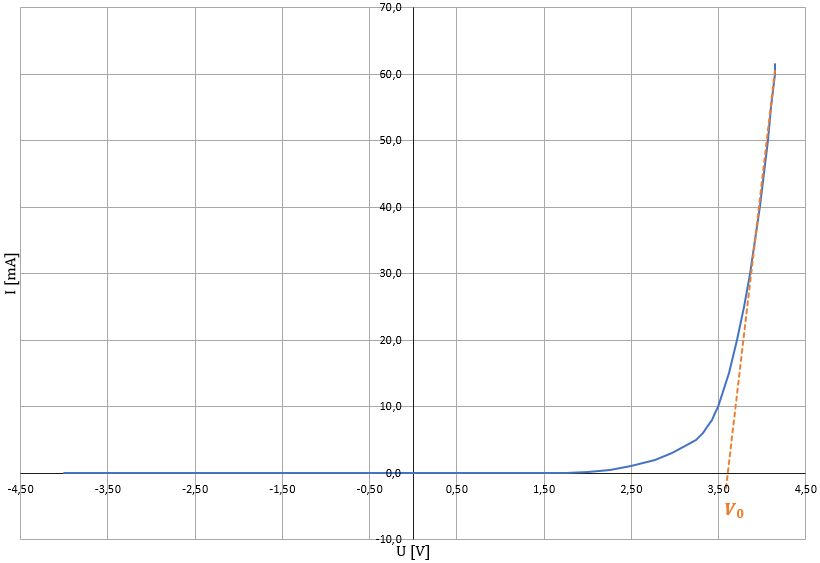
\includegraphics[width=\textwidth]{Fizyka104Wykres1}
		\end{figure}
	
		\begin{figure}[H]
			\centering
			\caption{Charakterystyka jasna, mniejsze natężenie oświetlenia}
			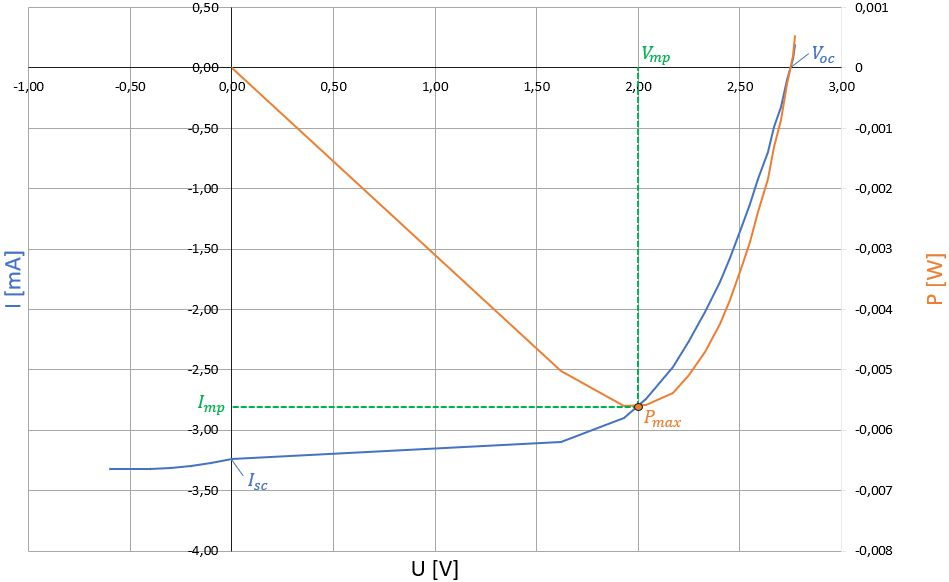
\includegraphics[width=\textwidth]{Fizyka104Wykres2}
		\end{figure}
	
		\begin{figure}[H]
			\centering
			\caption{Charakterystyka jasna, większe natężenie oświetlenia}
			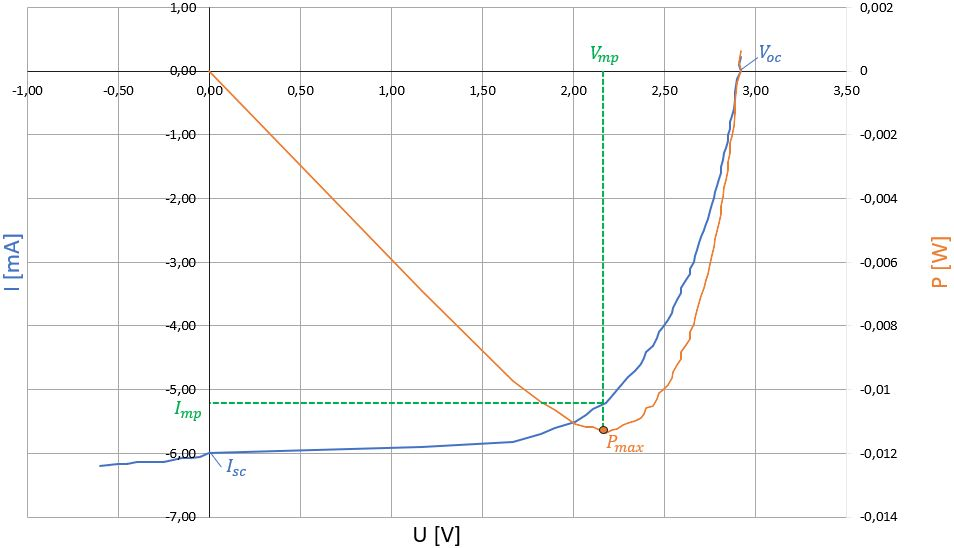
\includegraphics[width=\textwidth]{Fizyka104Wykres3}
		\end{figure}
		
	\section{Ostateczne wyniki}
		Ostateczne wyniki wraz z zaokrągleniami:
		\begin{description}[align=right,labelwidth=13cm]
			\item [Potencjał wbudowany:] {\((3,60\pm 0,17)V\)}
			\item [Współczynnik wypełnienia przy mniejszym natężeniu oświetlenia:] {\((63,1\pm 8,4)\%\)}
			\item [Współczynnik wypełnienia przy większym natężeniu oświetlenia:] {\((64,8\pm 8,3)\%\)}
		\end{description}
	
	\section{Dyskusja i wnioski}
		Narysowane zostały 3 wykresy charakterystyk I-V - charakterystyka ciemna, jasna przy mniejszym natężeniu oświetlenia oraz jasna przy większym natężeniu oświetlenia.
		Wyliczony potencjał wbudowany jest prawdopodobnie nieco niższy od prawdziwego, ponieważ maksymalny zmierzony prąd zestawem pomiarowym wynosił jedynie \(61,6mA\). Wyznaczony współczynnik wypełnienia ogniwa jest równy \((64,8\pm 8,3)\%\), co wskazuje na to, iż było to ogniwo niskiej klasy (60-70\%).
	\section{Literatura}
	\begin{enumerate}[label={[\arabic*]}]
		\item http://www.instsani.pl/513/parametry-pracy-paneli-pv
		\item http://www.sanwa-meter.co.jp/prg\_data/goods/img/PH41338255778.pdf, str.22-23
	\end{enumerate}
\end{document}